\documentclass[1pt]{extarticle}
\usepackage[utf8]{inputenc}
\usepackage{cite}
\usepackage{graphicx}
%ADDED BY FARZAD
\usepackage{subfig}
\usepackage[margin=1in,nomarginpar]{geometry}
\usepackage{subfig}
\usepackage{graphicx}
\usepackage{epsfig}
\usepackage{dblfloatfix}
\usepackage{xcolor}
\usepackage{hyperref}

\title{Implementation, Demonstration and Comparison of AC-Supplied and DC-Supplied Electrolysers in P834 Laboratory}
\author{S. A. Gorji, F. Farajizadeh}
\date{Mar 2020}


%check fig caption/label DONE
%figs efficiency graph {changing conventional module to conventional setup} DONE
%check electrolyser data sheet DONE
%revise 1.1.
\begin{document}

\maketitle

There are three steps to be conducted in this project:

\begin{itemize}
  \item \textbf{Step 0:}~ The rationale of proposing DC- supplied electrolysers;
  \item \textbf{Step 1:}~ Modular converter topologies for DC-supplied electrolysers;
  \item \textbf{Step 2:}~ Fault-tolerant converter topologies for DC-supplied electrolysers.
\end{itemize}

In this abstract proposal, the road-map required for \textbf{step 0} is briefly explained as below.

\section{A comparison between AC- and DC- supplied electrolysers}

\subsection{Justification}
As per the market demand, most of the commercial electrolysers such as ITM\cite{ITM}, Nel\cite{Nel} and Enapter\cite{Enapter} are AC-supplied, i.e. an on-board inverter is incorporated in their package to convert the grid-side AC input to the usable DC voltage for the electrolyser stack. However, with the dominance of renewable power sources such as solar photo-voltaic (PV) and battery storage systems, there is a significant need to introduce commercial DC-supplied electrolysers. In this study, we intend to use a low-power AC-supplied electrolyser\cite{QL500}  as a case-study and compare two main scenarios of AC-supplied electrolysers and DC-supplied electrolysers when they are connected to a DC power source. 


\subsection{Contributions}

\begin{figure}[h]
	\centering
	{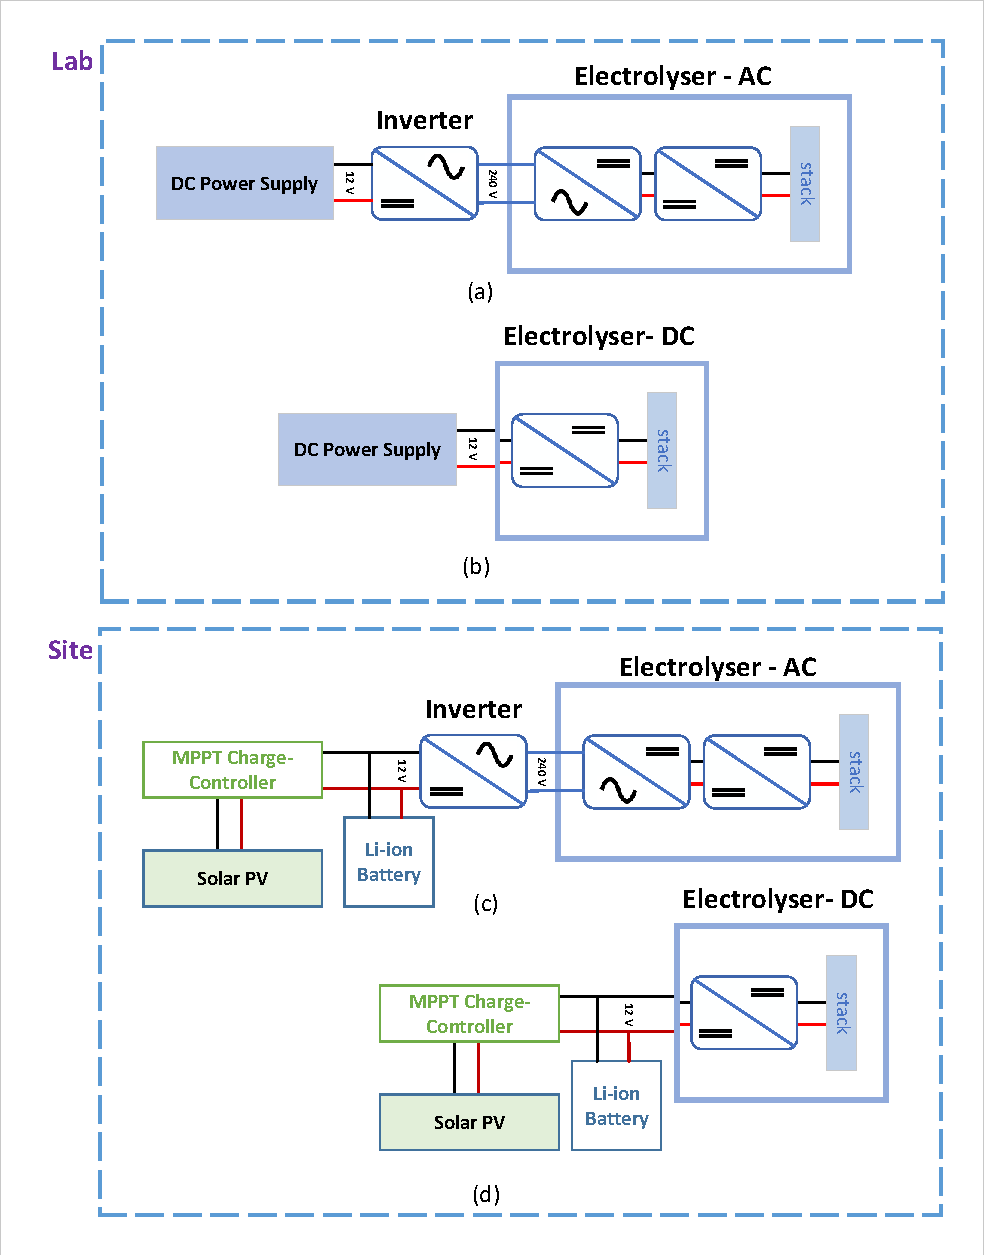
\includegraphics[width=0.68\textwidth]{images/LabSite.pdf}}
	\caption{Converting an AC Electrolyser to DC required for Step 0.}
	\label{labsite}
\end{figure}

As illustrated in Fig.~\ref{labsite}, the core idea is to propose a DC-supplied electrolyser for renewable energy sources to increase the efficiency and reliability of the system and reduce its net cost. Towards this aim, the proposed electrolyser together with the conventional AC-supplied electrolyser will be demonstrated and compared in the lab. Then as it is shown in Fig.~\ref{F_FIG1}, the same approach is followed on-site for both the proposed and conventional setups while they are fed with Solar PV panels and equipped with energy maximum power point tracker and storage systems to show the feasibility and credibility of the proposed system in a realistic situation.  

\subsubsection{Price}

As it is shown in Fig.~\ref{F_FIG1}(a), the conventional AC supplied electrolysers need an external inverter when they are connected to a DC supply. This arrangement causes unnecessary power losses in the external inverter and the electrolyser internal rectifier. It also increases the overall price of the system and decreases the reliability of the overall system due to the several energy conversion steps.
Therefore, in the proposed approach the electrolyser module is modified to be directly fed from the provided DC supply. In another terms, as shown in Figs.~\ref{labsite}(b) and (d) and Fig.~\ref{F_FIG1}(a), the external inverter and internal rectifier are merged into a simple DC to DC converter located inside the electrolyser. This way, the energy conversion stages of the whole system is scaled down into only three stages (instead of five stages), Fig.~\ref{F_FIG2}(b). \textbf{Therefore, the overall efficiency of the system will be significantly increase. This technique also decreases the overall price and physical size of the system, and owing to its less complexity, it provides a more reliable scheme to generate $\textrm{H}_2$.}  


\subsubsection{Efficiency}

According to the previous section, as the power conversion stages are reduced from three to one, the system efficiency will be improved. This is elaborated in Fig.~\ref{F_FIG2}, where the breakdown of the total loss for the proposed scheme (Fig.~\ref{F_FIG2}(b)) confirms the losses associated with the inverter and rectifier are eliminated. 


\begin{figure}[h!]
    \begin{center}
    \subfloat[]{
        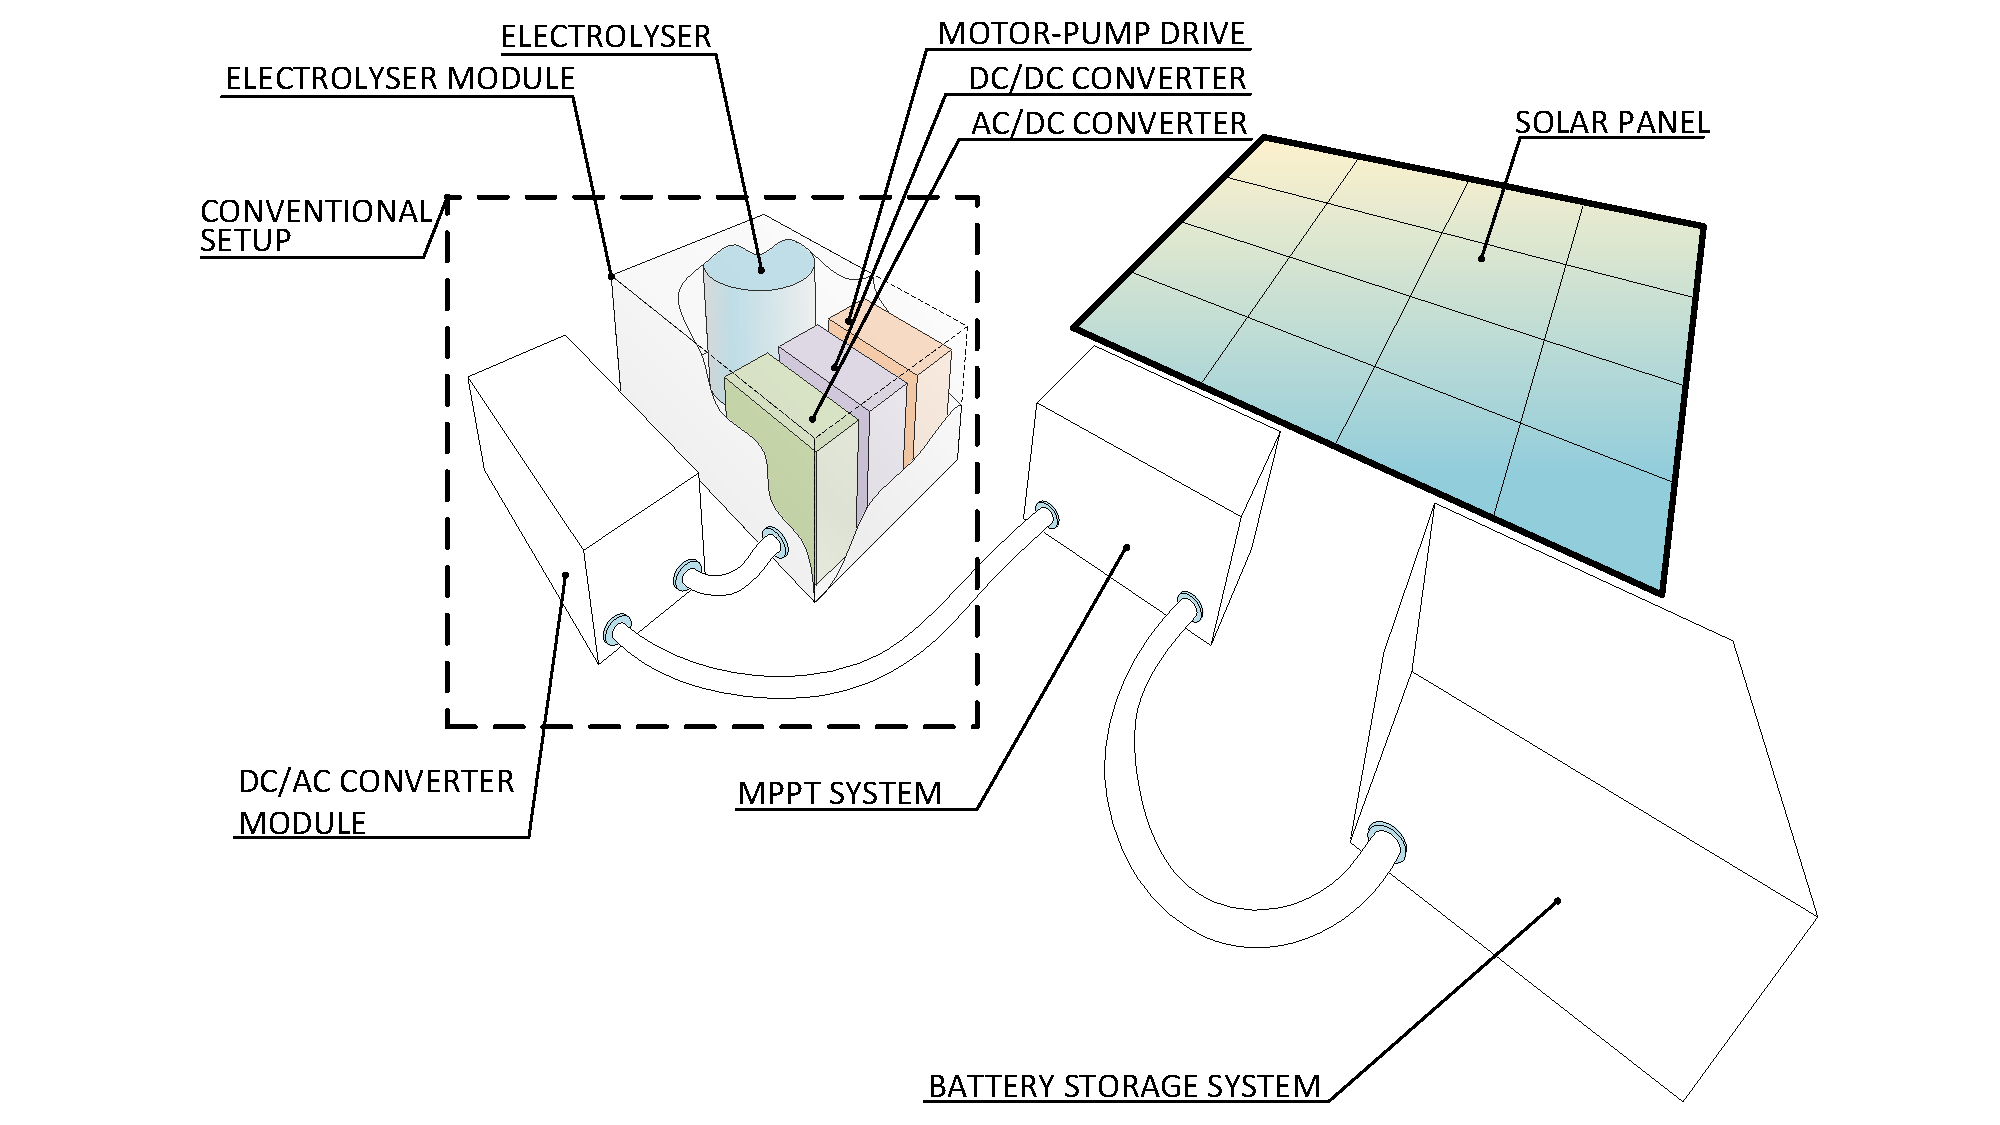
\includegraphics[clip, trim=3cm 0cm 3cm 0cm, width=0.7\linewidth]{images/F_FIG1A.pdf}
    }\\
    \subfloat[]{
        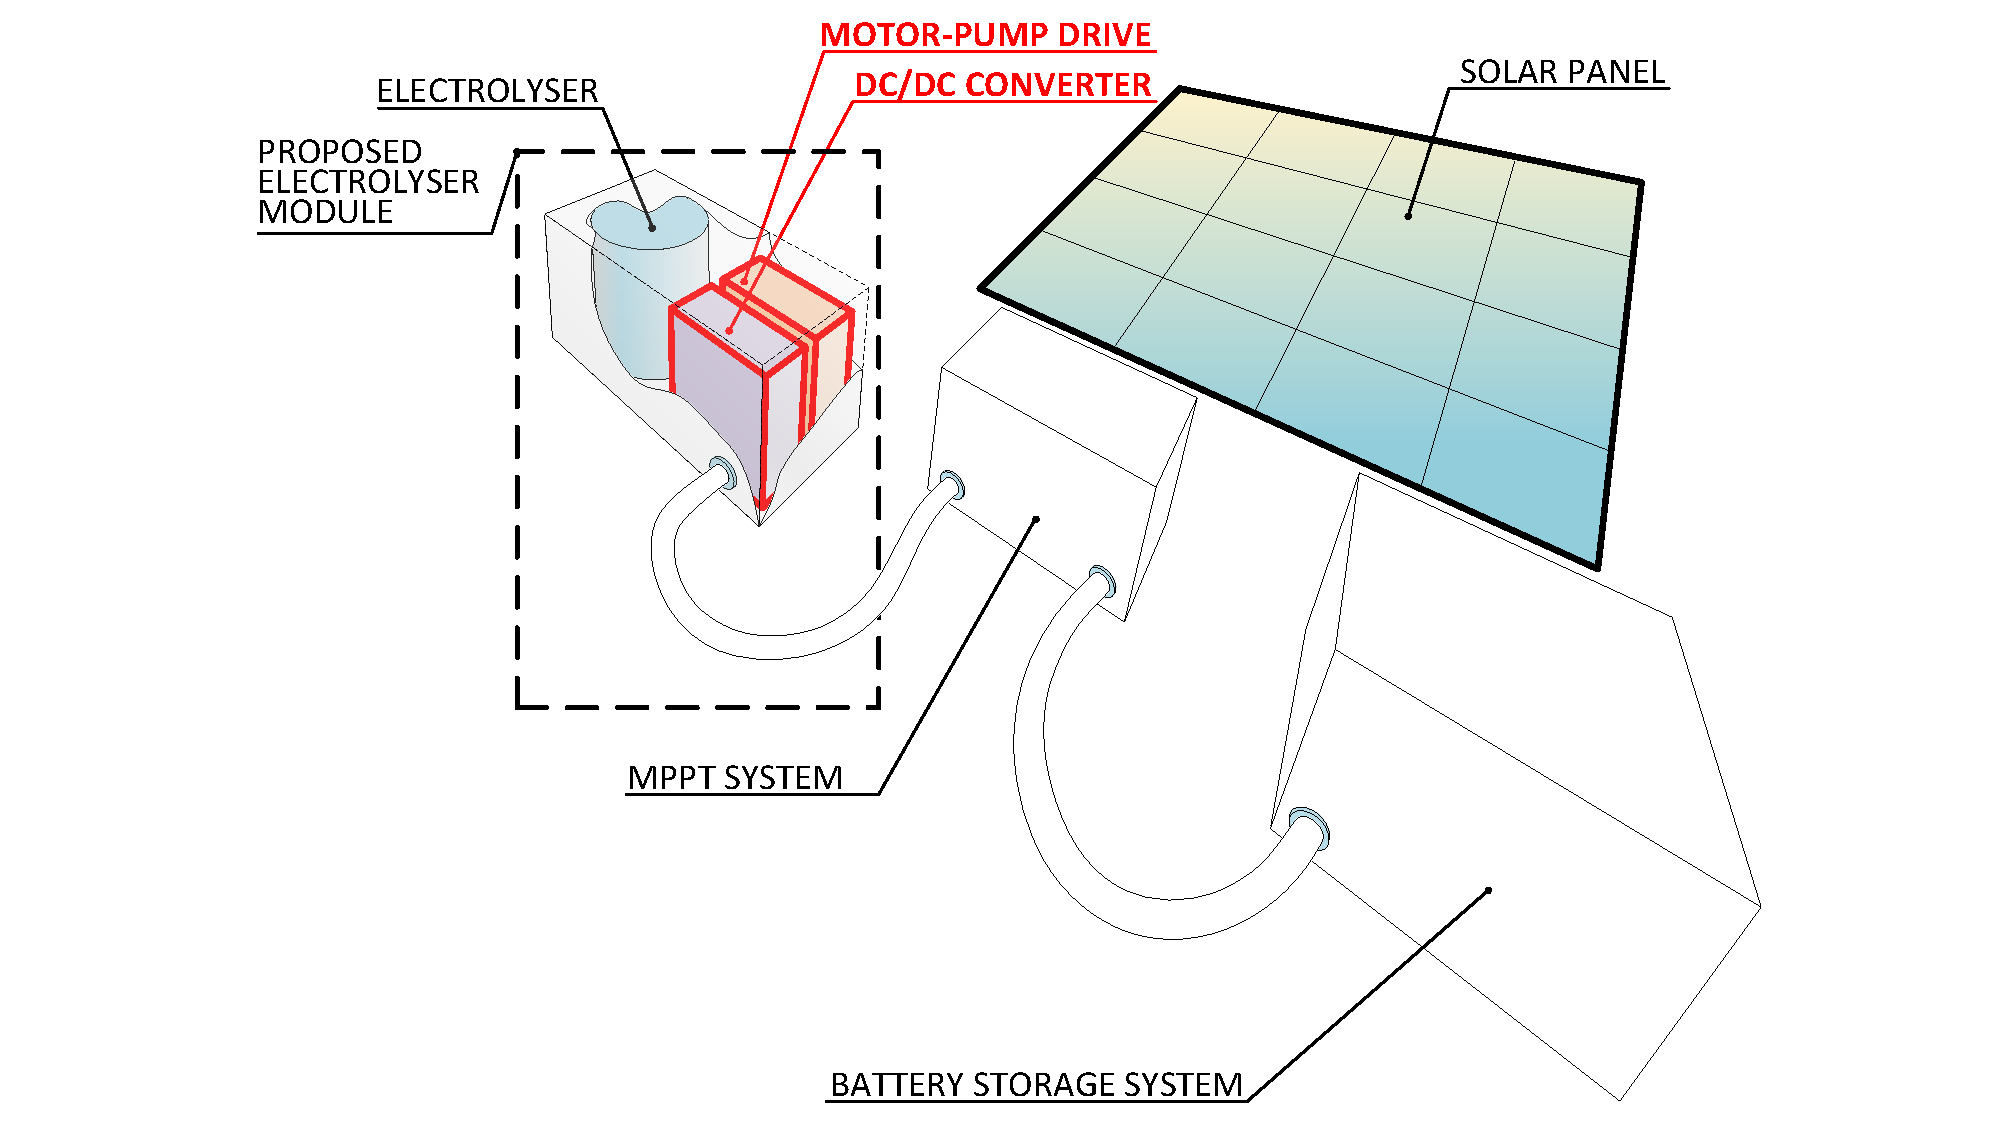
\includegraphics[clip, trim=3cm 0cm 3cm 0cm, width=0.7\linewidth]{images/F_FIG1B.pdf}
    }
    \caption{Photo-voltaic electrolyser systems; (a) conventional systems and (b) proposed system.}
    \label{F_FIG1}
    \end{center}
\end{figure}

\subsubsection{Future Demand}
 
The power generation systems are inevitably changing towards renewable energy sources, which affirms the DC power sources including PV panels are going to be the dominant future source of power. This would require an overarching revisit of the current infrastructure i.e. transition from centralised AC power plants to decentralised DC power generation systems. In another words adaption of the manufacturing industry to introduce DC-friendly products such as DC-supplied electrolysers unavoidable.    
 
\subsection{Demonstration}

In order to demonstrate the proposed idea and compare it with the conventional approach (shown in Fig.~\ref{labsite}), the proposed system (DC electrolyser module) together with it conventional counterpart (AC electrolyser module) are to be exposed by replacing its casing with a transparent box in the indoor demonstration, probably similar to what is shown in Fig.~\ref{F_FIG1}. For outdoor demonstration, the conventional electrolyser and other systems involved will remain intact and they are used according to the required standards. Moreover, for the proposed electrolyser a proper casing (similar to the conventional system) will be designed and used to make the prototype as comparable as possible to the conventional system. This way, on the one hand, the electrical performance of both systems can be carefully controlled and investigated in indoor tests, and, on the other hand, the realistic operation of the systems in different weather conditions can be studied and compared.


\begin{figure} [t!]
    \begin{center}
    \subfloat[]{
        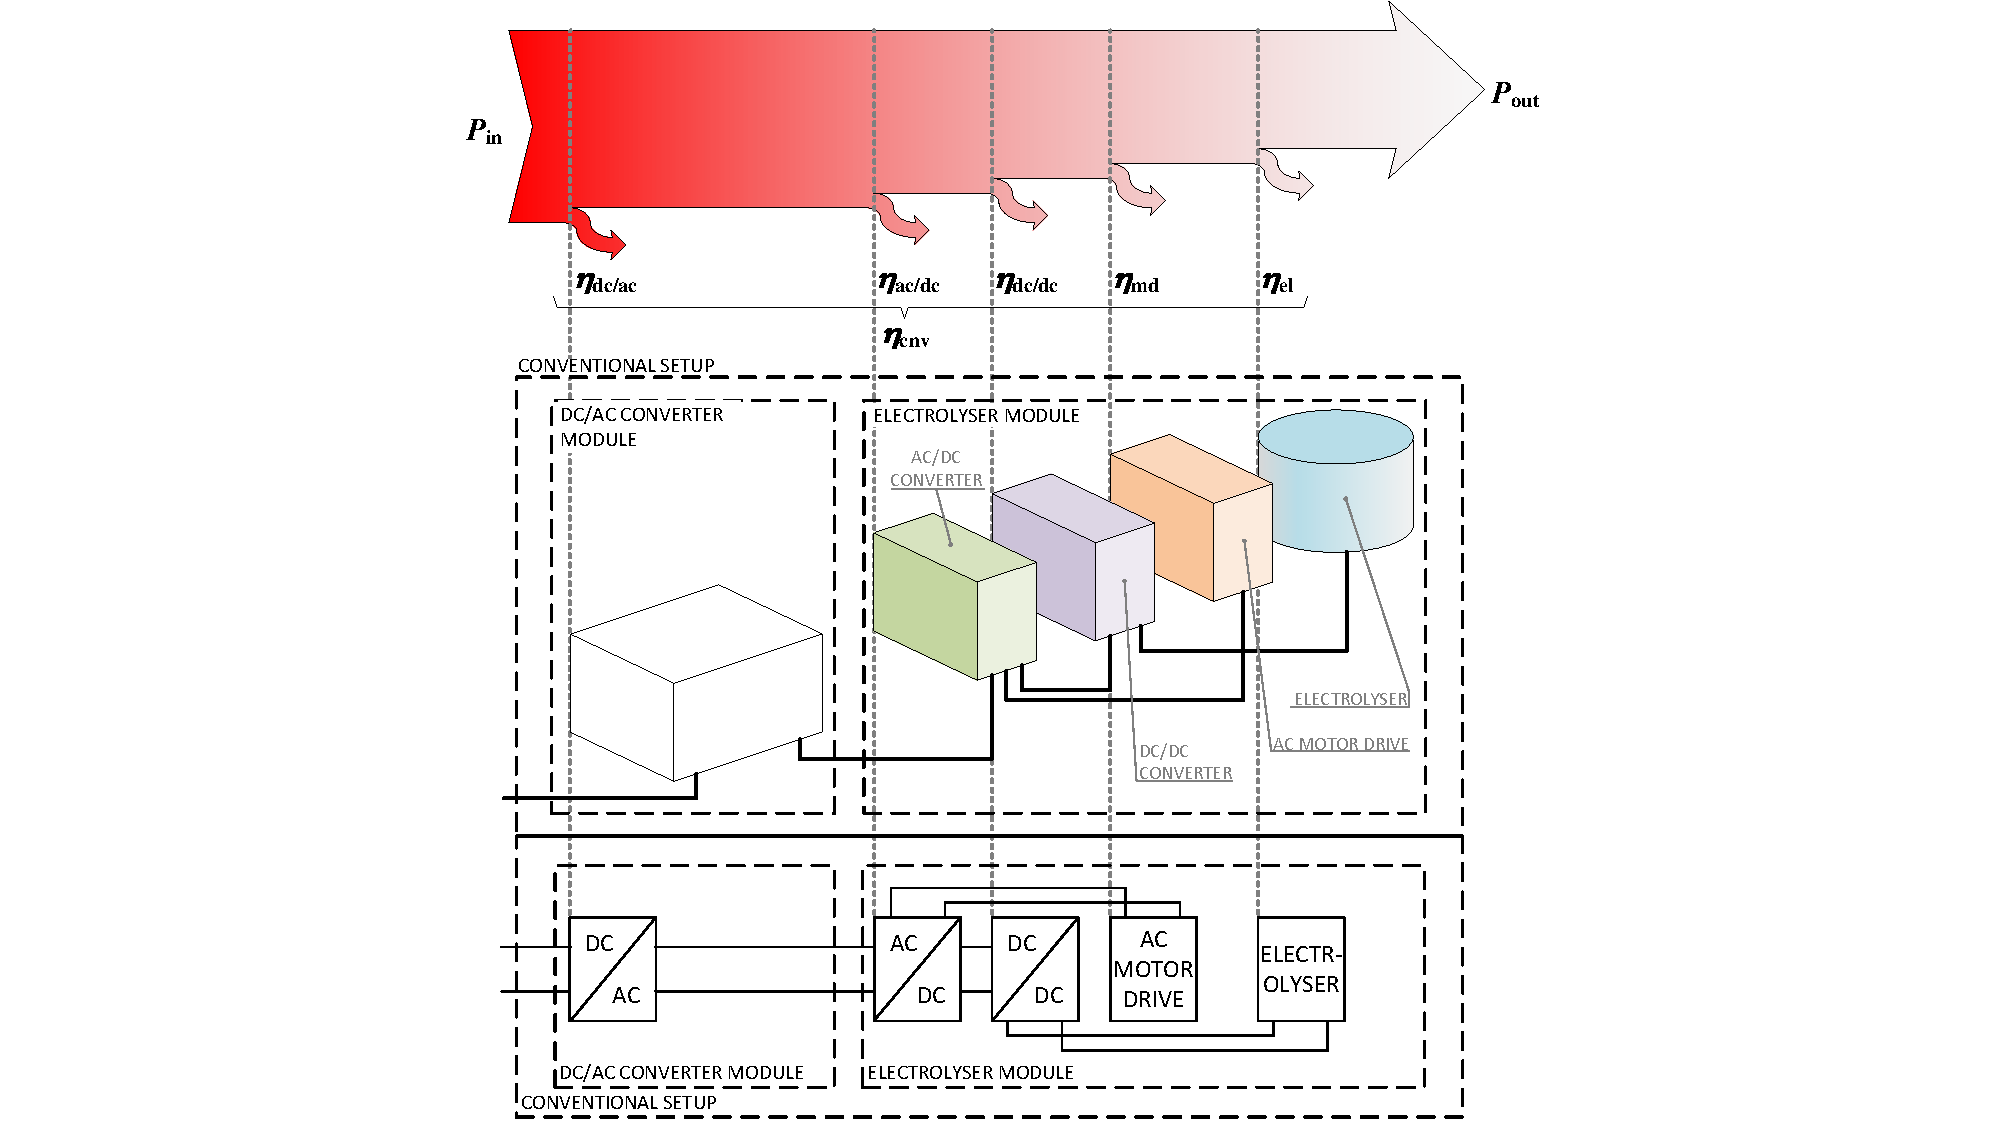
\includegraphics[clip, trim=7.8cm 0cm 7.8cm 0cm, width=0.602\linewidth]{images/F_FIG2A.pdf}
    }
    \subfloat[]{
        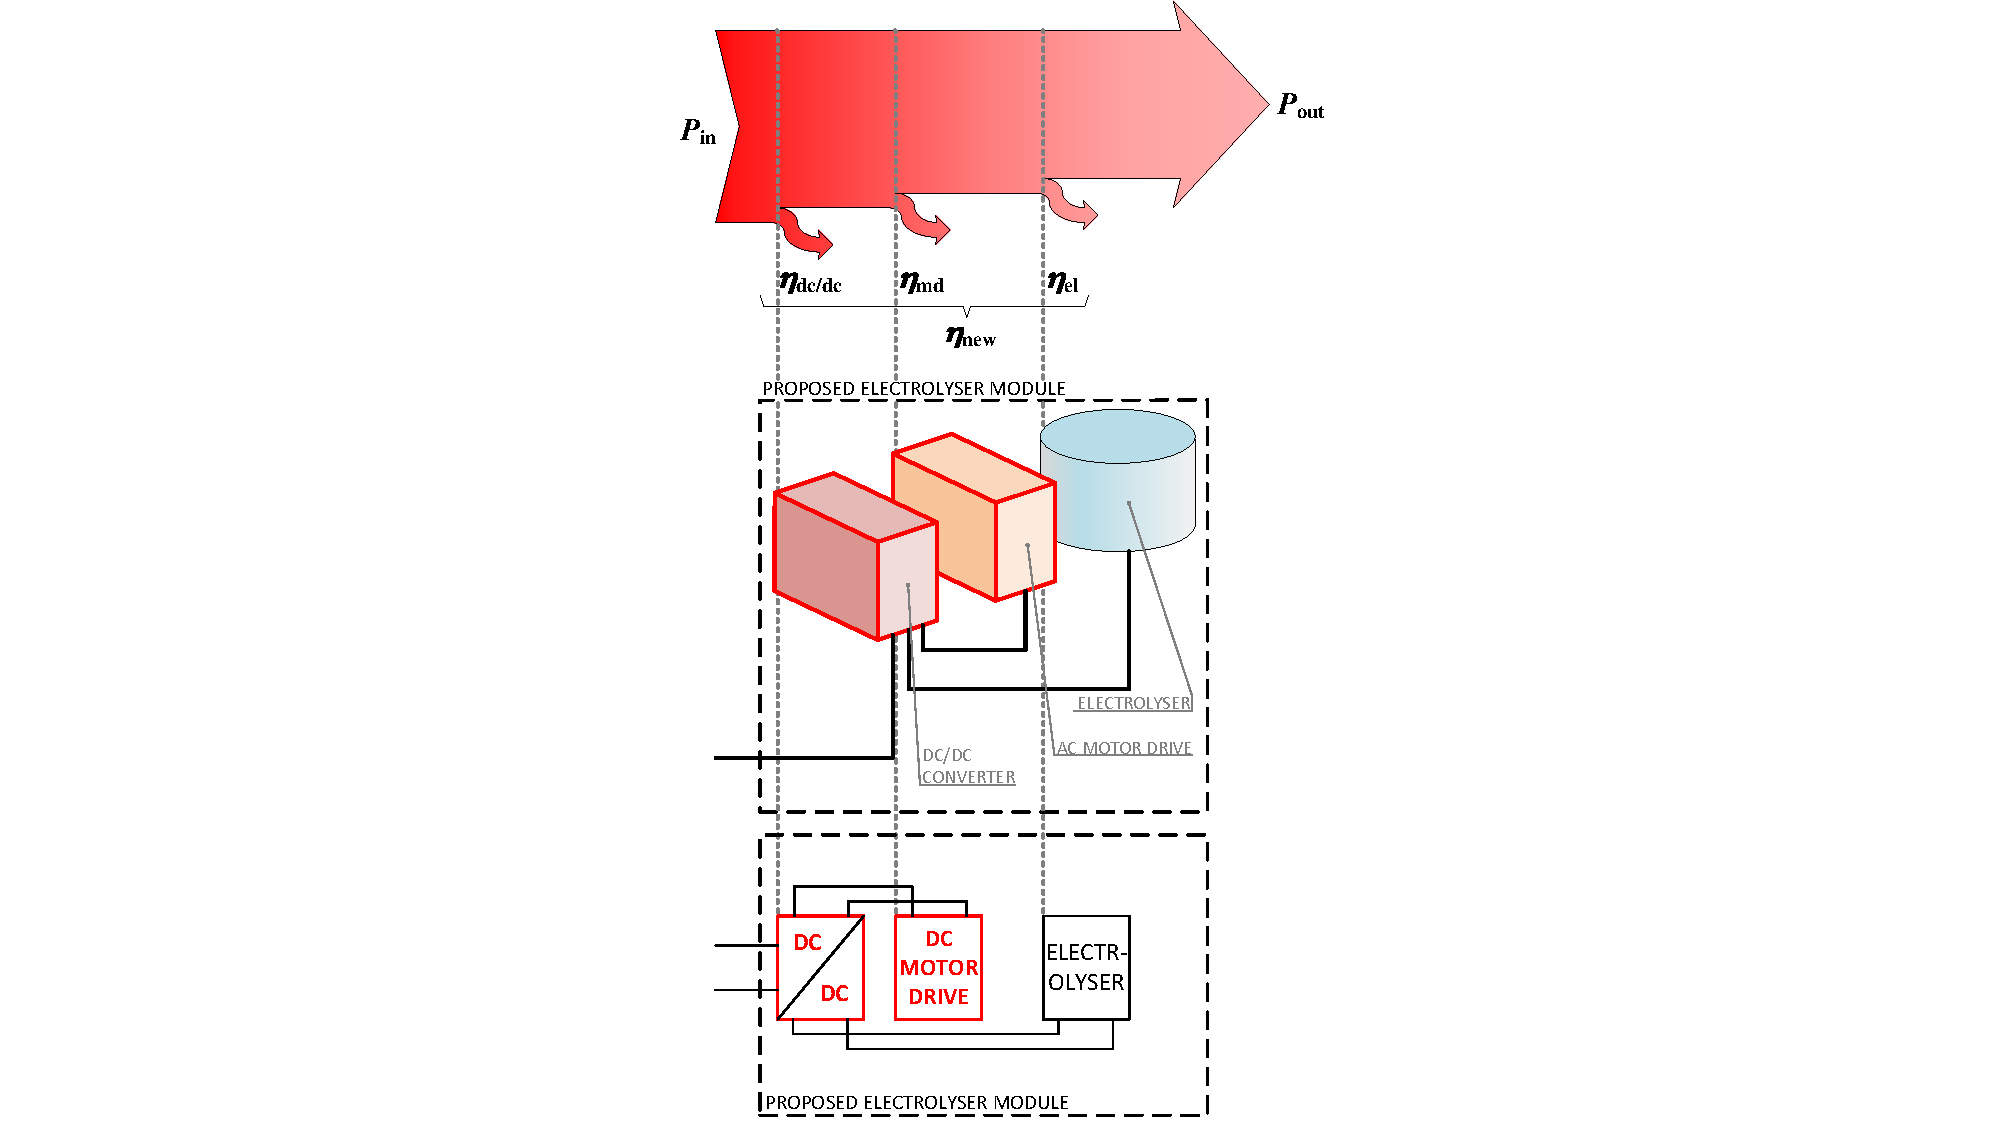
\includegraphics[clip, trim=10.91cm 0cm 10.91cm 0cm, width=0.398\linewidth]{images/F_FIG2B.pdf}
    }
    \caption{Power diagram for photo-voltaic electrolyser systems; (a) conventional systems and (b) proposed system.}
    \label{F_FIG2}
    \end{center}
    \vspace{-0.5cm}
\end{figure}

\subsection{Deliverable}
To make a credible report on the operation of both conventional and the proposed systems, following steps are going to be taken.

\begin{itemize}
\item Prepare the demonstrative indoor and outdoor setups.
\item Arrange a complete and reasonable list of measurement components to observe the environmental and electrical variables (such as humidity, temperature, light intensity, input power, and output power).
\item Prepare a comprehensive test sheet consisting of all necessary data required for indoor and outdoor efficiency and reliability investigations.
\item Arrange frequent and long-term measurements and probation to investigate the operation of both setups in different weather condition and record the data.
\item Prepare a written deliverable data obtained from the indoor and outdoor tests.
\item Organize the indoor and outdoor setups for the on-site inspections.
\end{itemize}

\subsection{Cost Estimation and Timeline for Step 0}
As shown in Fig.~\ref{F_FIG2}, two electrolysers will be demonstrated in P834 lab (one AC-supplied and one DC-supplied setup). It is worth noting that the existing equipment will assist to reduce the project cost. The equipment used in the final setup will also be used in other prospective projects. Therefore, the required and existing equipment for the indoor tests are listed in Tables \ref{TBL1} and \ref{TBL2}, respectively. According to the table below, the requested budget at this stage is 10k AUD. In addition, there are existing equipment that should be used to fulfill this step and are valued 20.5k AUD. Hence, the overall price for the equipment used in this project is 30.5k AUD. Moreover, the required period of time to finish Step 0 is estimated two months, which is elaborated in Table~\ref{TBL3}.

%% TBL1
    \begin{table}[h!]
        \centering
        \caption{Cost Estimation for the Required Equipment.}
        \vspace{-2.5mm}
        \label{TBL1}
            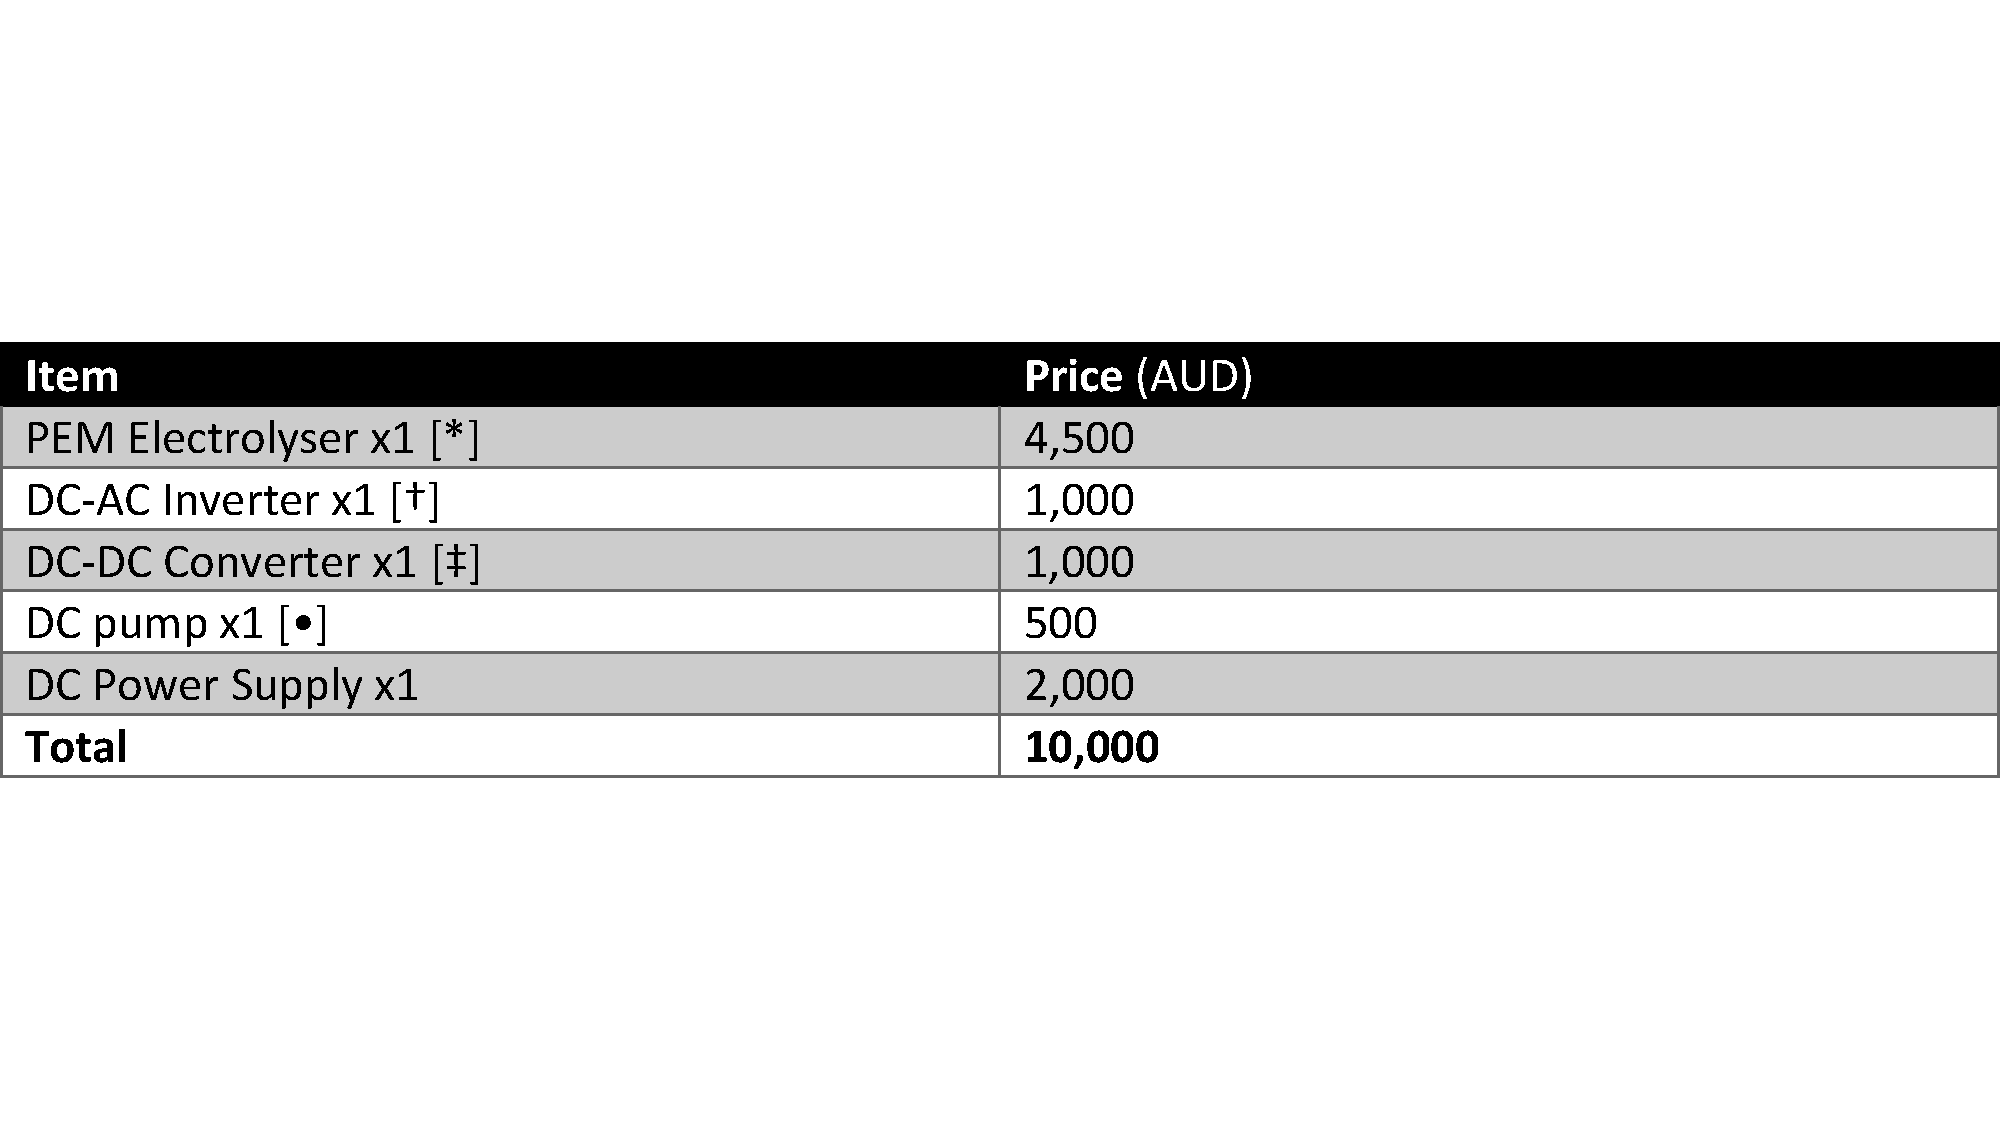
\includegraphics[clip,trim= 0cm 5.5cm 0cm 5.5cm,width=1\linewidth]{images/TBL1.pdf}
        \vspace{-6mm}
    \end{table}

%% TBL2
    \begin{table}[h!]
        \centering
        \caption{Value of the Existing Equipment.}
        \vspace{-2.5mm}
        \label{TBL2}
            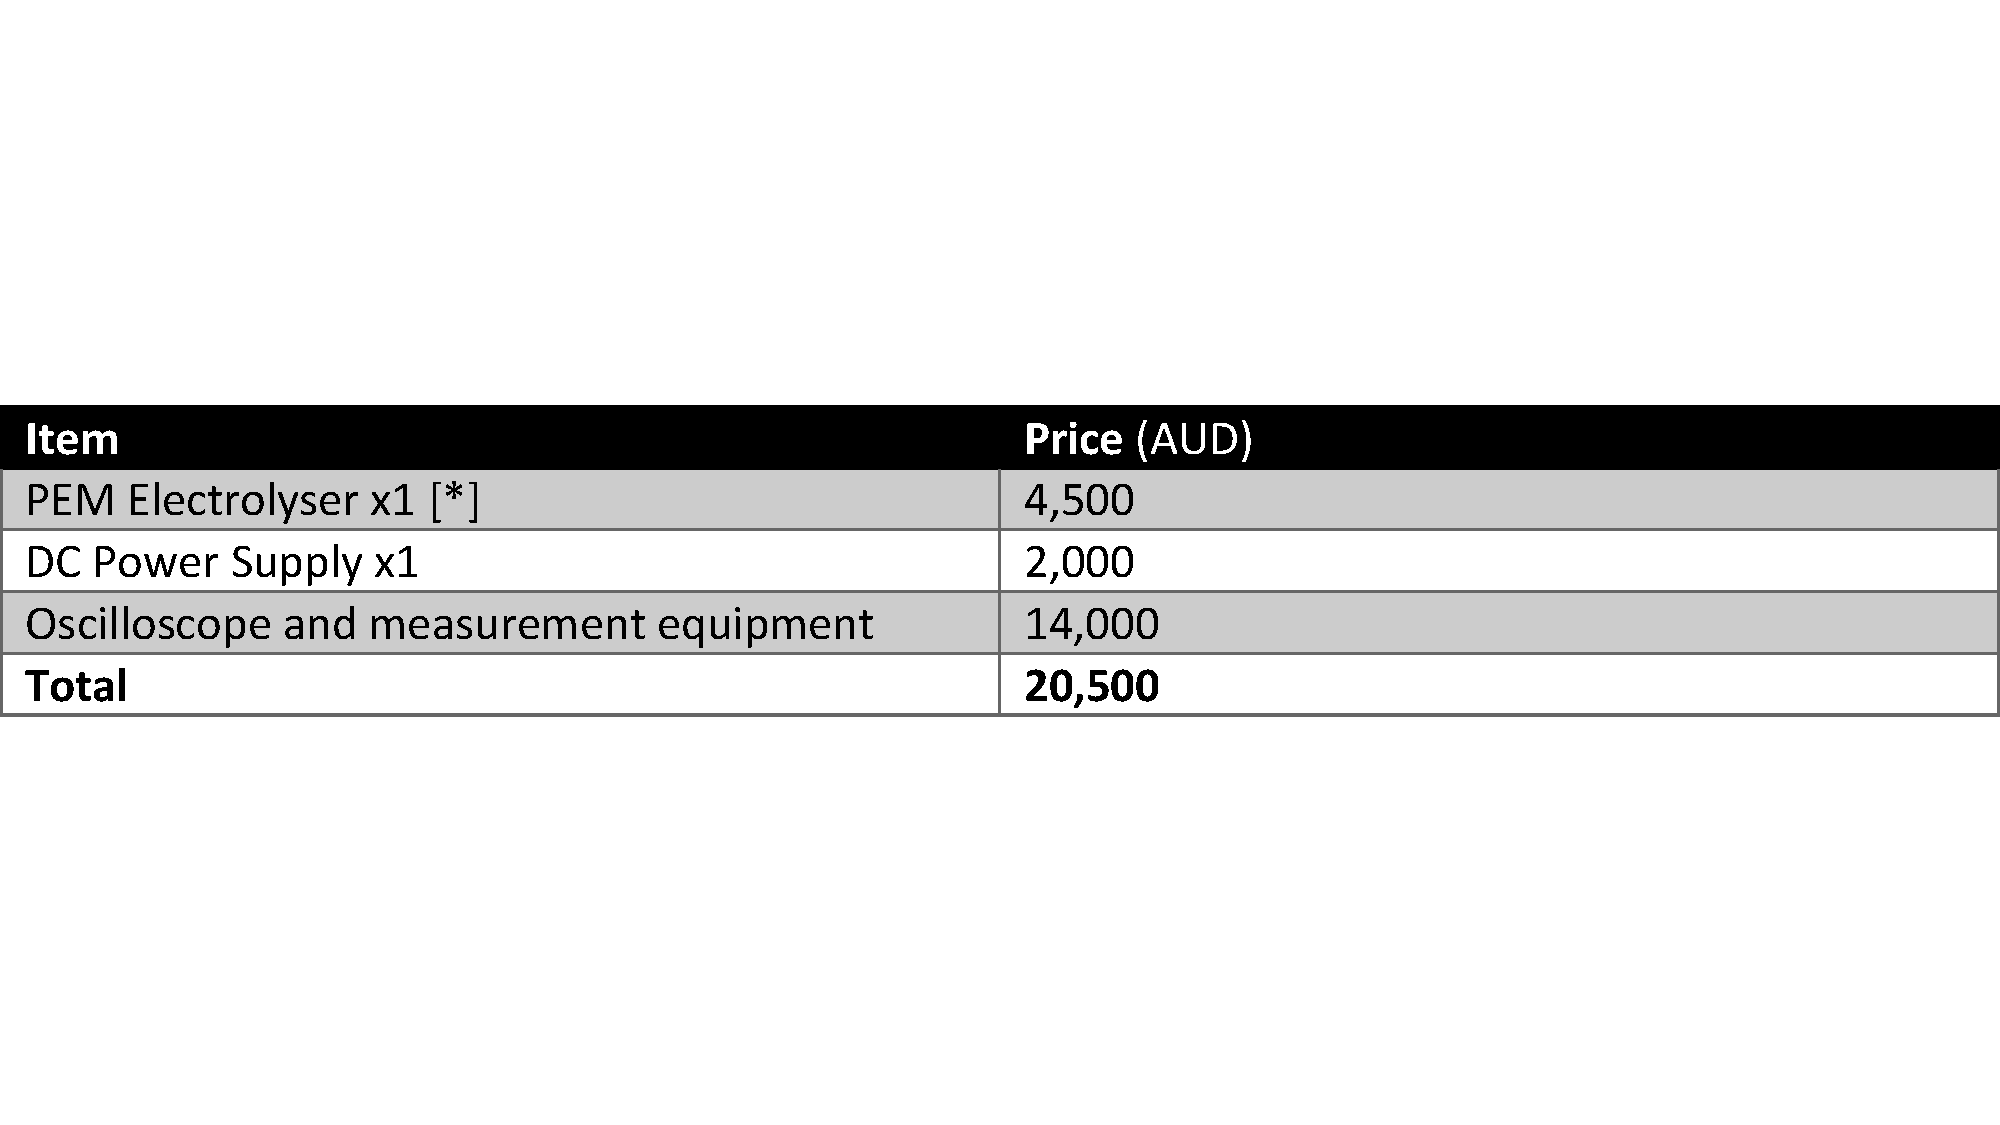
\includegraphics[clip,trim= 0cm 6.5cm 0cm 6.5cm,width=1\linewidth]{images/TBL2.pdf}
        \vspace{-6mm}
    \end{table}

Following, the links for each component is given.

\begin{itemize}
    \item [*] \href{https://www.fuelcellstore.com/hydrogen-equipment/laboratory-gas-generators/pem-hydrogen-generator-ql-500}{https://www.fuelcellstore.com/hydrogen-equipment/laboratory-gas-generators/pem-hydrogen-generator-ql-500}
    \item [\dagger] \href{https://www.victronenergy.com/inverters/phoenix-inverter-vedirect-250va-800va}{https://www.victronenergy.com/inverters/phoenix-inverter-vedirect-250va-800va}
    \item [\ddagger] \href{https://www.victronenergy.com/dc-dc-converters}{https://www.victronenergy.com/dc-dc-converters}
    \item [\bullet] \href{https://www.pumpwarehouse.com.au/12v-dc-diaphragm-pumps/}{https://www.pumpwarehouse.com.au/12v-dc-diaphragm-pumps/}
\end{itemize}

%% TBL3
    \begin{table}[h!]
        \centering
        \caption{The Project Timeline.}
        \vspace{-2.5mm}
        \label{TBL3}
            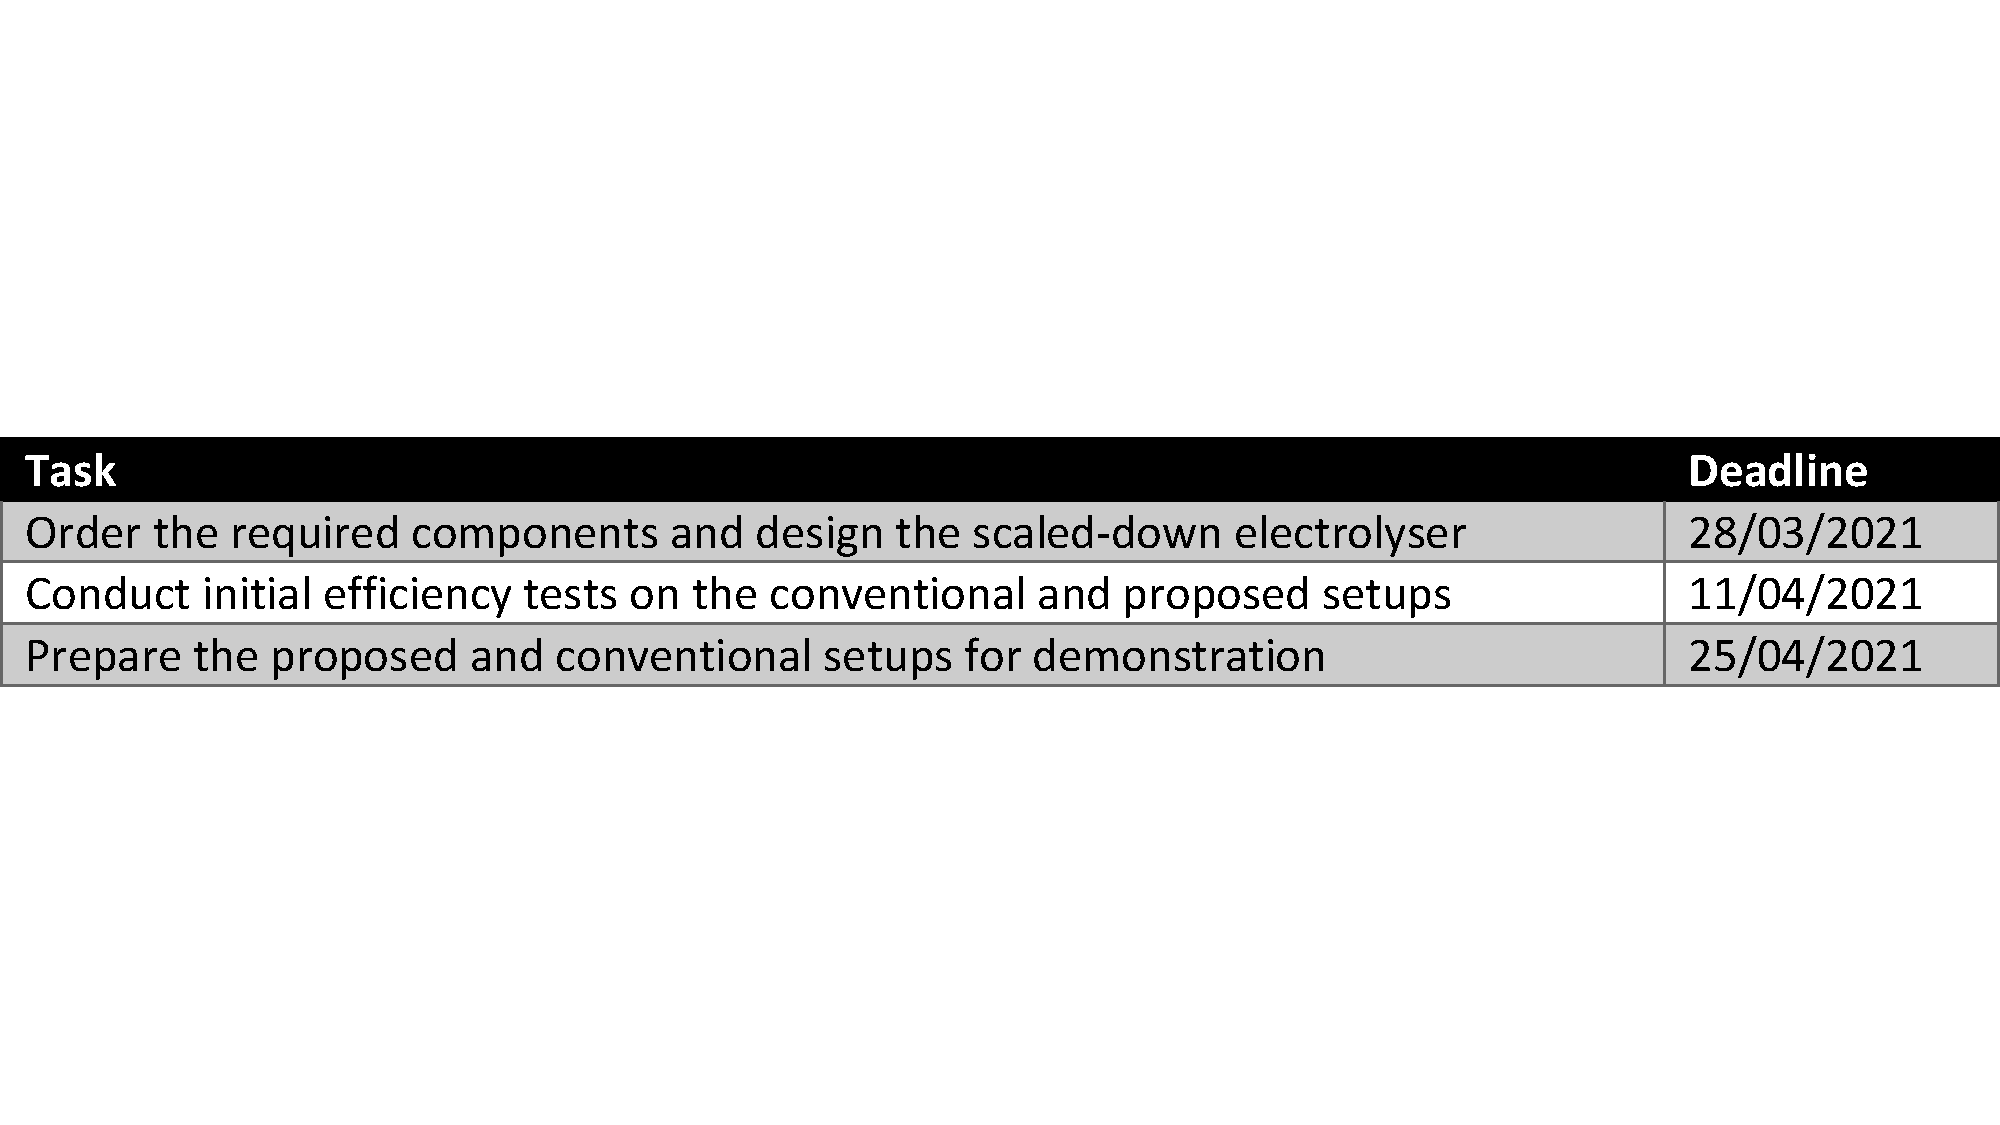
\includegraphics[clip,trim= 0cm 7cm 0cm 7cm,width=1\linewidth]{images/TBL3.pdf}
        \vspace{-6mm}
    \end{table}

\pagebreak

\bibliographystyle{ieeetr}
\bibliography{mybib}
\end{document}
